\documentclass{article}
\usepackage[utf8]{inputenc}
\usepackage{titling}
\usepackage{graphicx}
\usepackage{xcolor}
\usepackage[colorlinks=true,linkcolor=darkgray, urlcolor =gray]{hyperref}
\usepackage[spanish]{babel}
\DeclareUnicodeCharacter{301}{~}
\usepackage{url}
\DeclareUnicodeCharacter{202F}{\,}


\title{Práctica 4: Doble servidor virtual:\\Sitio 1: Web dinámica MySQL y PHP\\Sitio 2: Apache con Wordpress}
\author{Cristina Díaz García}
\date{Enero 2019}

\renewcommand\maketitlehooka{\null\mbox{}\vfill}
\renewcommand\maketitlehookd{\vfill\null}


\begin{document}

\addcontentsline{toc}{section}{Índice general}

\begin{titlingpage}
\maketitle

\begin{center}

\includegraphics[scale=2]{apache.jpg} 
\end{center}

\end{titlingpage}

\newpage

\tableofcontents

\newpage

\section{Sitio 1: Web dinámica MySQL y PHP}

Inicialmente, se instala Apache con el gestor de paquetes, apt en nuestro caso (\textit{apt install apache2}). Añadimos la dirección IP de nuestra máquina (\textit{ServerName 127.0.0.1}) a nuestro fichero de hosts (\textit{/etc/apache2/apache2.conf}. Tras eso, podemos proceder a iniciar el servicio (\textit{service apache2 start}). Activamos el módulo cgi (\textit{a2enmod cgi}) y reiniciamos el servicio de apache (\textit{service apache2 restart}).

A continuación creamos el directorio para crear el dominio virtual diaz.garcia.com (\textit{mkdir -­p /var/www/diaz.garcia.com/html}). Volvemos al archivo de hosts y añadimos nuestro dominio (\textit{nuestra IP(varía según la red a la que nos conectemos, por lo que tendríamos que cambiarlo al cambiar de red) diaz.garcia.com\\nuestra IP(varía según la red a la que nos conectemos, por lo que tendríamos que cambiarlo al cambiar de red) www.diaz.garcia.com}). También crearemos la configuración de nuestro host en /etc/apache2/sites-available, copiando como borrador la configuración por defecto (\textit{cp 000­default.conf diaz.garcia.com.conf}). Modificamos este archivo y configuramos el nombre del servidor, el alias (para poder usar www.diaz.garcia.com) y el directorio desde el que empezará a buscar:

\begin{flushleft}
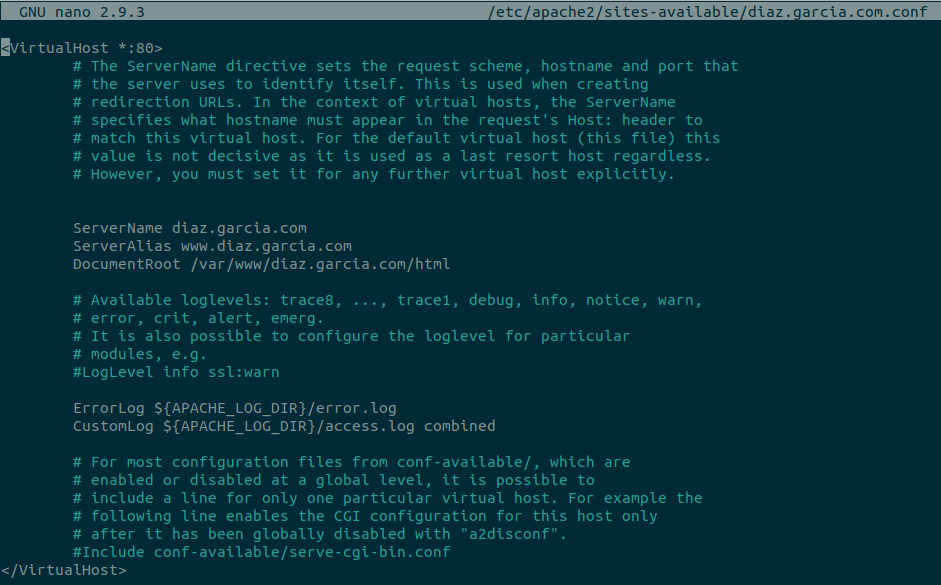
\includegraphics[scale=0.37]{conf.png}
\end{flushleft}

Activamos el host (\textit{a2ensite diaz.garcia.com.conf}) y recargamos el servicio de Apache (\textit{service apache2 reload}).

Procedemos a instalar el intérprete de PHP y librerías que necesita (\textit{apt install php libapache2-mod-php php-­mysql php-­gettext php-­mbstring}). Creamos un archivo de prueba de PHP en \textit{/var/www/diaz.garcia.com/html/index.php}, reiniciamos el servicio (\textit{service apache2 restart}) y comprobamos que funciona.

Copiamos todos los archivos proporcionados en el directorio de nuestro servidor (\textit{/var/www/diaz.garcia.com/html}).

\begin{flushleft}
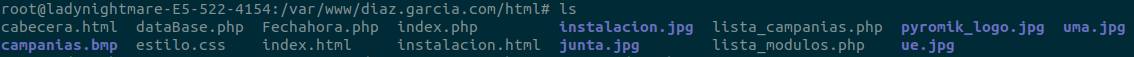
\includegraphics[scale=0.3]{dir.png}
\end{flushleft}

Instalamos MySQL (\textit{apt install mysql-server}) y lo instalamos de forma segura, ejecutando \textit{mysql\_secure\_instalation}. Haciendo uso del cliente de mysql, cambiamos el método de acceso para root a \textit{mysql\_native\_password}. 

Descargamos la última versión de phpmyadmin de la \href{https://www.phpmyadmin.net/files/}{web oficial} y descomprimimos los archivos en \textit{/var/www/html}, la renombramos como phpmyadmin y cambiamos los permisos para que su propietario y el grupo sea \textit{www-data}, para que así phpmyadmin pueda acceder desde el navegador como \textit{http://\textbf{miIP}/phpmyadmin}, aunque en mi caso, por la configuración realizada es \textit{http://\textbf{miIP}/index.php}. Si no funcionara, habría que comprobar que los permisos fueran los adecuados.

Ya sea con el cliente o en la web, ejecutamos los script proporcionados para crear las tablas e introducir los datos.

Una vez hecho todo esto, deberíamos tener algo parecido a lo siguiente:

\begin{flushleft}
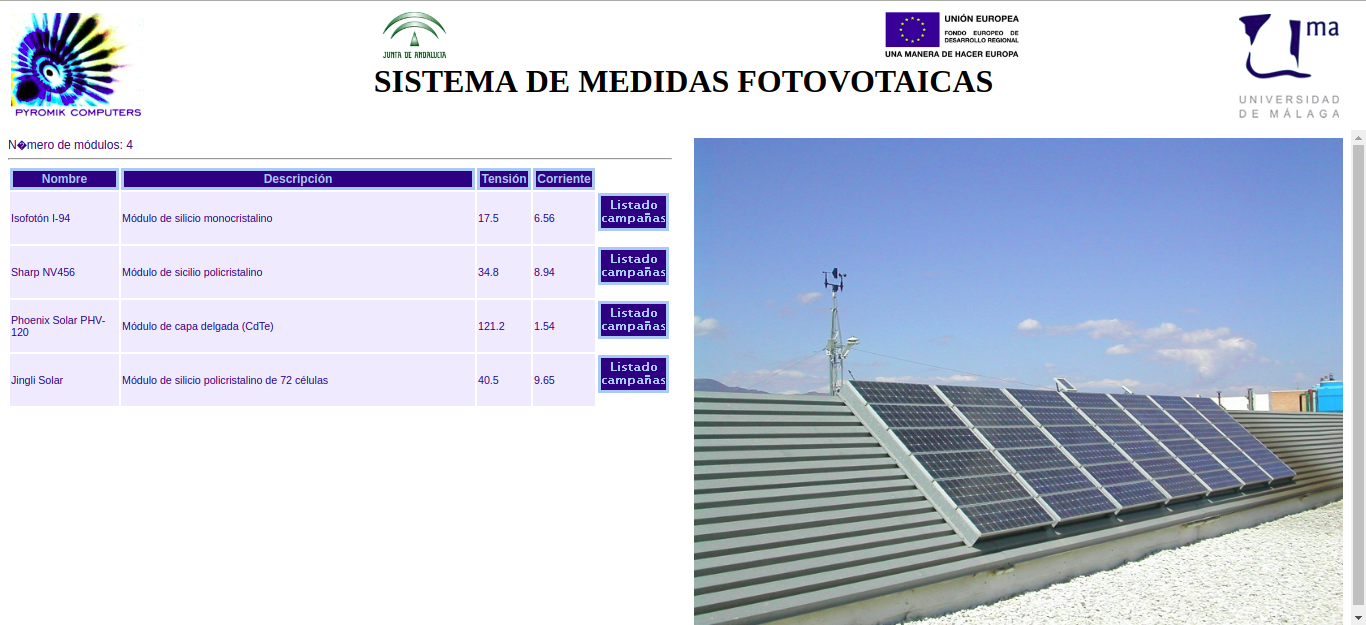
\includegraphics[scale=0.27]{fotovoltaico.png}
\end{flushleft}

\begin{flushleft}
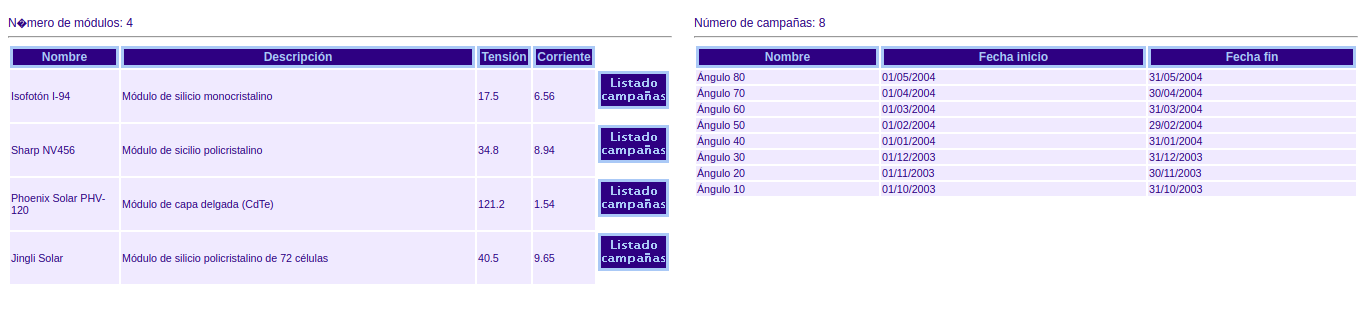
\includegraphics[scale=0.27]{consulta.png}
\end{flushleft}

\section{Sitio 2: Apache con Wordpress}

Intalamos la última versión de Wordpress de la página oficial (\textit{wget https://wordpress.org/latest.tar.gz} y la descomprimimos en \textit{/var/www/html/phpmyadmin} y cambiamos los permisos para que su propietario y el grupo sea \textit{www-data}.

En \textit{http://\textbf{miIP}/index.php} creamos el usuario wordpress y la tabla con el mismo nombre, y empezamos la configuración.

\begin{flushleft}
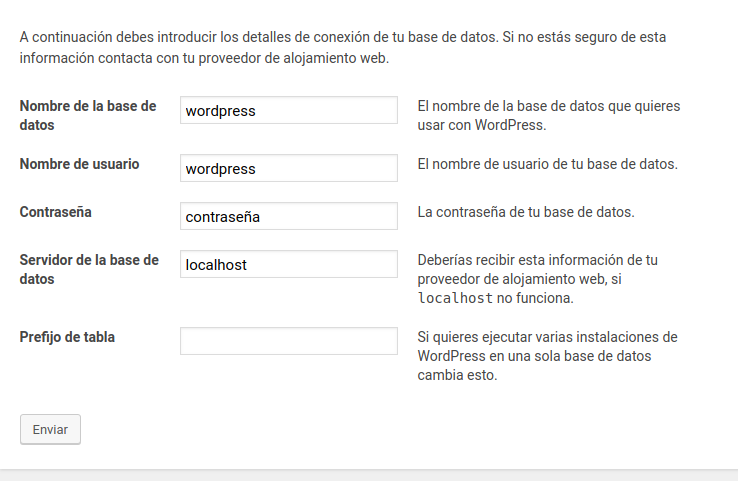
\includegraphics[scale=0.5]{wp.png}
\end{flushleft}

Seguimos con la instalación...

\begin{flushleft}
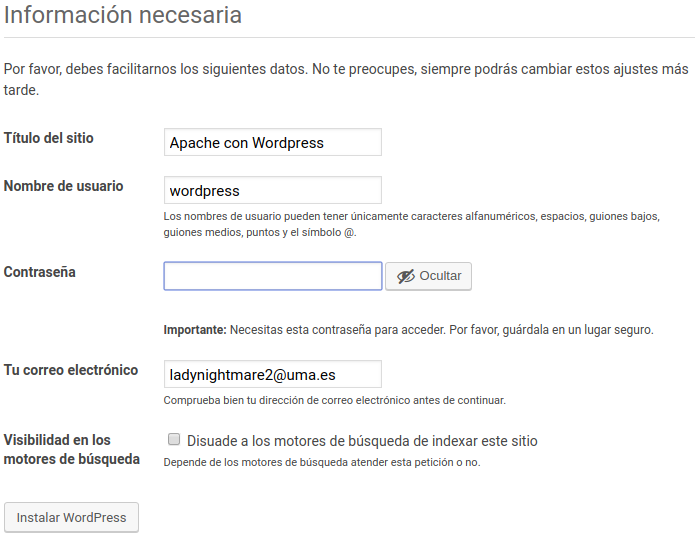
\includegraphics[scale=0.5]{wordpress.png}
\end{flushleft}

A continuación creamos el directorio para crear el dominio virtual diaz.garcia.es (\textit{mkdir -­p /var/www/diaz.garcia.es/html}). Volvemos al archivo de hosts y añadimos nuestro dominio (\textit{nuestra IP(varía según la red a la que nos conectemos, por lo que tendríamos que cambiarlo al cambiar de red) diaz.garcia.es\\nuestra IP(varía según la red a la que nos conectemos, por lo que tendríamos que cambiarlo al cambiar de red) www.diaz.garcia.es}). También crearemos la configuración de nuestro host en /etc/apache2/sites-available, copiando como borrador la configuración del ejercicio anterior (\textit{cp diaz.garcia.com.conf diaz.garcia.com.conf}). Modificamos este archivo y configuramos el nombre del servidor, el alias (para poder usar www.diaz.garcia.es) y el directorio desde el que empezará a buscar:

\begin{flushleft}
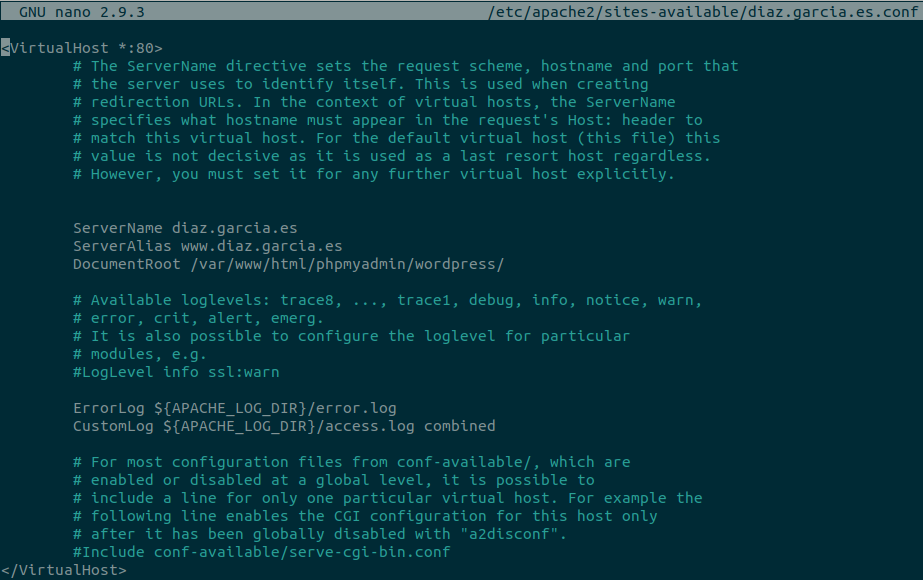
\includegraphics[scale=0.37]{conf2.png}
\end{flushleft}

Activamos el host (\textit{a2ensite diaz.garcia.es.conf}) y recargamos el servicio de Apache (\textit{service apache2 reload}).

Y ya tenemos listo nuestro blog wordpress al que acceder con \textit{http://\textbf{miIP}/wordpress/wp-admin/} y \textit{http://diaz.garcia.es/wp-login.php}.

\begin{flushleft}
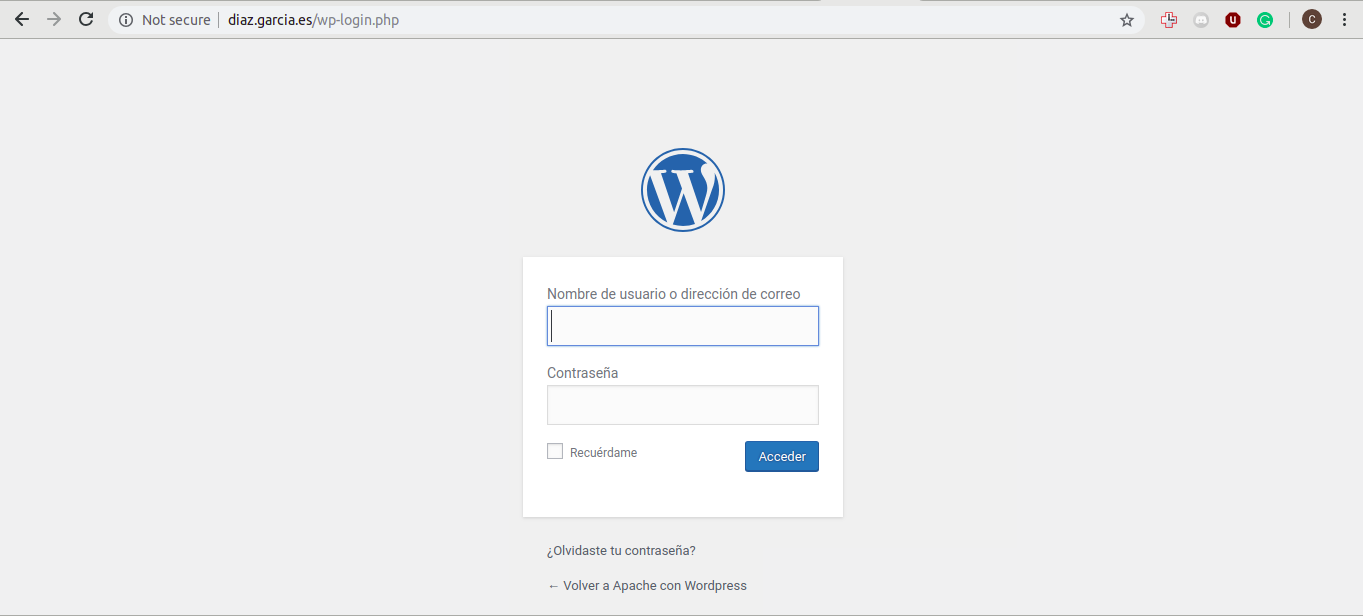
\includegraphics[scale=0.27]{wordp.png}
\end{flushleft}

\end{document}